%% LaTeX-Beamer template for KIT design
%% by Erik Burger, Christian Hammer
%% title picture by Klaus Krogmann
%%
%% version 2.4
%%
%% mostly compatible to KIT corporate design v2.0
%% http://intranet.kit.edu/gestaltungsrichtlinien.php
%%
%% Problems, bugs and comments to
%% burger@kit.edu

%% Class options
%%   aspect ratio options: 
%%   -- 16:9 (default)
%%   -- 4:3
%%   language options: 
%%   -- en (default)
%%   -- de
%%   position of navigation bar:
%%   -- navbarinline (default): bottom of the white canvas
%%   -- navbarinfooter : more compressed variant inside the footer
%%   -- navbarside : side bar at the left of the white canvas
%%   -- navbaroff : none
%% example: \documentclass[16:9,de,navbarinfooter]{sdqbeamer}
\documentclass[16:9,en,navbarinfooter]{sdqbeamer}

%% \documentclass{sdqbeamer} 

%% TITLE PICTURE

% if a custom picture is to be used on the title page, copy it into the 'logos'
% directory, in the line below, replace 'myimage' with the 
% filename (without extension) and uncomment the following line
% (picture proportions: 63 : 20 for standard, 169 : 40 for wide
% *.eps format if you use latex+dvips+ps2pdf, 
% *.jpg/*.png/*.pdf if you use pdflatex)

% \titleimage{myimage}

%% GROUP LOGO 

% for a custom group logo, copy your file into the 'logos'
% directory, insert the filename in the line below and uncomment it

\grouplogo{transparent}

% (*.eps format if you use latex+dvips+ps2pdf,
% *.jpg/*.png/*.pdf if you use pdflatex)

%% GROUP NAME

% for groups other than SDQ, please insert in the line below and uncomment it
% \groupname{My group}

% the presentation starts here 

\title{Efficient Pruning of N-gram Corpora for Culturomics using Language Models}
\subtitle{}
\author{Caspar Nagy}

% Bibliography 
\usepackage{booktabs}
\usepackage{longtable}
\usepackage{color}
\usepackage{array}
\usepackage{algorithm}
\usepackage{algpseudocode}
\usepackage{pgfplots}
% \pgfplotsset{compat=1.15}
 \usepgfplotslibrary{groupplots}
\usepackage{subcaption}
\usepackage{pdflscape}
\usepackage{diagbox}
\usepackage{multicol}
\DeclareUnicodeCharacter{2212}{−}
\usepgfplotslibrary{groupplots,dateplot}
\usetikzlibrary{patterns,shapes.arrows}
\pgfplotsset{compat=newest}
\usepackage[citestyle=authoryear,bibstyle=numeric,hyperref,backend=biber%,style=verbose
]{biblatex}
\addbibresource{presentation.bib}
\bibhang1em
\usepackage{listings}
\begin{document}

%title page
\KITtitleframe{}

%table of contents

\section{Motivation}
\subsection{Culturomics}
\begin{frame}[fragile]{Motivation}
\vspace{1cm}
\begin{columns}
\column{.6\textwidth}
\begin{itemize}
    \item Part of Digital Humanities
    \item Culturomics uses Big Data Technology to observe Culture over hundreds of years.
    \item N-gram corpora made from historic books, news articles, 
        law text, \ldots
    \item The ``Google Books Ngrams'' is the most relevant corpus.
        \begin{itemize}
            \item Based on the Google Books Project
            \item $\approx 4\%$ off all books ever written
            \item All consecutive word chains (N-grams) up to length 5 were counted up by year
            \item Over 2TB in size
        \end{itemize}
\end{itemize}

    \textbf{How can we reduce the size of corpora like this?}\\
\column{.4\textwidth}
    \begin{center}
    \tiny
        Example 1-gram Analysis by the original Google Books Ngrams Paper \textbf{[Michel2012]}
    \end{center}
    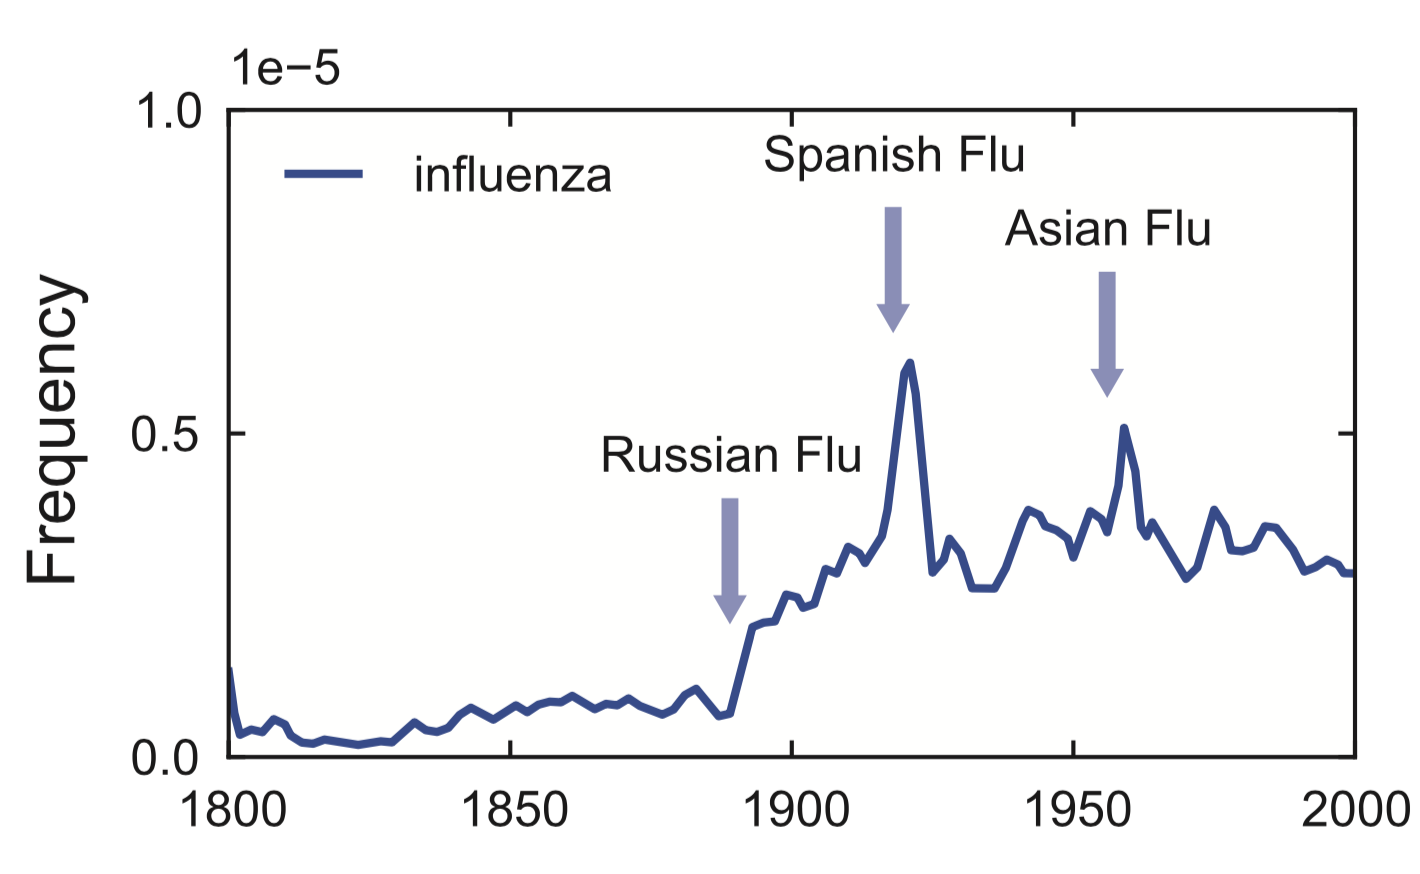
\includegraphics[width=\linewidth]{influenza}
        %\vspace{.5cm}
%    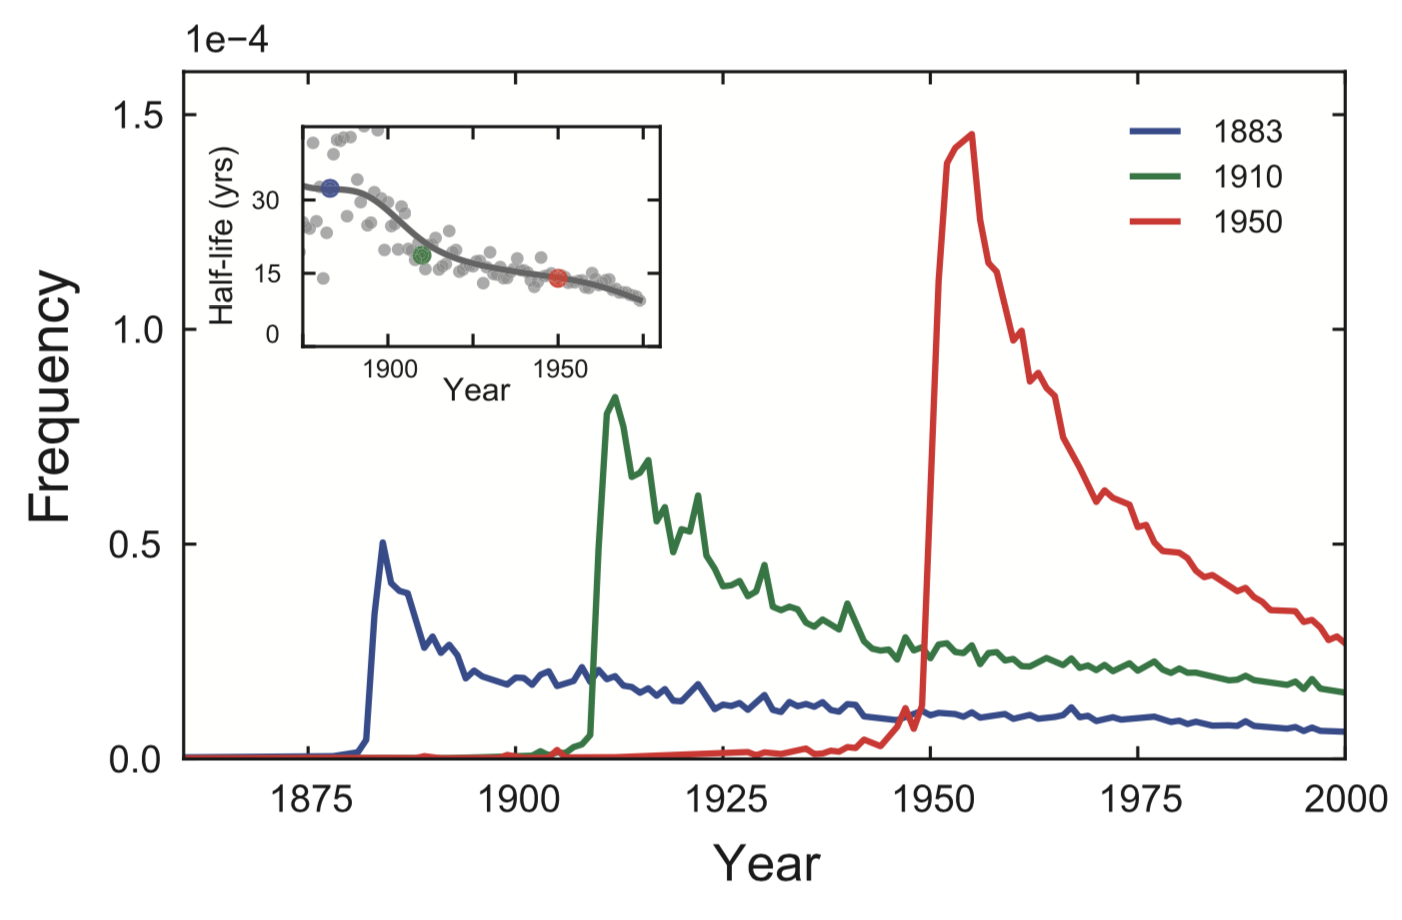
\includegraphics[width=.8\linewidth]{years}
\lstset{
frame = single,  
framexleftmargin=1pt}
\begin{lstlisting}[title={Sample of 2-grams.tsv}]
Last	Departure	80
law	restored	1639
\end{lstlisting}
% Later	Virginia	160
% lake	area		106
\end{columns}
\end{frame}
\subsection{N-gram Corpora}
\begin{frame}[fragile]{Culturomics and Natural Language Processing (NLP)}
\begin{itemize}
    \item NLP uses comparable N-gram corpora
    \item NLP uses probablistic methods to process human language
    \begin{itemize}
        \item Speech Recognition (``their'' vs. ``they're'')
        \item Grammar Checking 
        \item Topic Grouping 
    \end{itemize}
    \item They have two main ways to reduce their size:
    \begin{itemize}
            \item Compression
            \item Pruning
    \end{itemize}
    \item We will focus on pruning.
        \begin{itemize}
                \item Calculate some score $f(w)$ over each N-gram 
                \item Delete all N-grams where $f(w) < \theta$ for some $\theta \in \mathbb R$
                \item Example: Prune all N-grams that have a count < 40 (frequency pruning)
        \end{itemize}
\end{itemize}
\end{frame}

\section{N-gram NLP}
\subsection{N-gram NLP} 

\begin{frame}{N-gram Language Models}
\vspace{1.1cm}
    Let history $h:= (Alice\ went\ to\ the\ door\ and)$, word $w:=(knocked)$.
\begin{itemize}
\item Estimating Probabilities:
    $$P(knocked|Alice\ went\ to\ the\ door\ and) \overset {MLE} = \frac {Count(Alice\ went\ to\ the\ door\ and\ knocked)}{
Count(Alice\ went\ to\ the\ door\ and)}$$

\item Markov-assumption:
\begin{equation*} 
\begin{split}
    P(w|h) = P(knocked|Alice\ went\ to\ the\ door\ and )
    & \approx P_{3-gram}(w|h) =  P(knocked|              door\ and) \\
&  \approx P_{2-gram}(w|h) =  P(knocked|                    and) \\
&  \approx P_{1-gram}(w|h) =  P(knocked) \\
\end{split}
\end{equation*}

\item Chain Rule of Probability for longer Text: $P(w_1,\ldots, w_n)=\prod_{k=1}^n P(w_k|w_1, \ldots, w_{k-1})$
\item Backoff
    \begin{itemize}
            \item N-gram models cannot capture examples of every word combination
            \item $P(w|h)=0$ both unrealisitic and undesireable
                \begin{itemize}
                    \item if $P(w|h) = 0$, fall back to a shorter model
                \end{itemize}
    \end{itemize}
\end{itemize}
\end{frame}

\begin{frame}{NLP Pruning}
\vspace{1cm}
\begin{itemize}
%   \item Pruning is an effective way to reduce the size of an N-gram corpus.
    \item Scoring Functions used:
    \begin{itemize}
        \item Frequency: $Count(w)$
        \item Weighted difference: $Count(w) \cdot (\log(P_{original}(w)) - \log(P_{backed\ off}(w)))$%~(\cite{seymore1996})
            \begin{itemize}
                \item $P(City | York) \approx P(City | New\ York)$
            \end{itemize}
        \item Relative entropy (``Stolcke Pruning'')%~(\cite{Stolcke2000})
    \end{itemize}
    \item Problem: Culturomics is a research tool
    \begin{itemize}
        \item We want\dots
            \begin{itemize}
            \item clear semantics: ``How does the data presentated relate to the raw data?''
            \item reliable counts.
            \item no backoff.
            \end{itemize}
        \item \textbf{This rules out all methods but frequency pruning.}
    \end{itemize}
\end{itemize}

\end{frame}

\section{A model-based Pruning Approach}
\subsection{A model-based Pruning Approach}

\begin{frame}{A model-based Pruning Approach}
    \begin{columns}
    \column{.6\textwidth}
    \begin{itemize}
        \item $P(w) \propto Count(w)$
        \item $P_{N-gram}(w) \approx P(w)$
        \item Use $P_{N-gram}(w)$ to estimate $Count(w)$ using a linear model
        \item Prune all N-grams for which our estimatation error 
            is $\leq r$ for some tolerance $r\in\mathbb N$
        \item Properties:
        \begin{itemize}
            \item uses shorter N-gram's information
            \item pruned counts are never off by more than $r$
            \item threshold pruning as a corner case for $slope=0,\ intercept = \frac r2$
        \end{itemize}
\end{itemize}
\column{.4\textwidth}
\begin{figure}
    % This file was created by tikzplotlib v0.9.3.
\begin{tikzpicture}

\definecolor{color0}{rgb}{0.12156862745098,0.466666666666667,0.705882352941177}

\begin{axis}[
width=\linewidth,
tick align=outside,
tick pos=left,
%caption={6-gram model},
x grid style={white!69.0196078431373!black},
xlabel={\(\displaystyle P_{6-gram}(w)\)},
xmin=-1.20562638805832e-07, xmax=1e-06,
xtick style={color=black},
y grid style={white!69.0196078431373!black},
ylabel={$Count(w)$}, %{\(\displaystyle C(w)\)},
ymin=0, ymax=20,
ytick style={color=black}
]
\addplot [only marks, mark=*, draw=kit-blue100, fill=kit-blue100, opacity=0.1, colormap/viridis]
table{%
x                      y
4.82289090640062e-08 1
4.82289090640062e-08 1
1.44686727192018e-07 3
4.82289090640062e-08 1
4.82289090640062e-08 1
4.82289090640062e-08 1
4.82289090640062e-08 1
3.50015711350592e-08 1
7.23433635960092e-08 2
4.8228909064006e-08 1
4.82289090640062e-08 1
9.64578181280124e-09 1
4.82289090640062e-08 1
4.82289090640061e-08 1
4.82289090640062e-08 1
4.82289090640062e-08 1
4.82289090640061e-08 1
4.82289090640062e-08 1
4.82289090640062e-08 1
4.82289090640062e-08 1
4.47466773626338e-08 1
4.82289090640061e-08 1
4.82289090640062e-08 1
4.82289090640062e-08 1
1.72246103800022e-09 1
4.41791533410743e-10 1
2.4114454532003e-08 1
4.82289090640062e-08 1
1.03347662280013e-07 3
4.82289090640061e-08 1
2.4114454532003e-08 1
4.82289090640061e-08 1
4.82289090640062e-08 1
4.82289090640062e-08 1
4.82289090640062e-08 1
4.82289090640061e-08 1
4.82289090640062e-08 1
9.64578181280122e-08 2
4.82289090640061e-08 1
4.82289090640062e-08 1
4.82289090640061e-08 1
4.82289090640061e-08 1
4.82289090640061e-08 1
4.82289090640061e-08 1
4.82289090640061e-08 1
4.82289090640061e-08 1
4.82289090640062e-08 1
4.82289090640062e-08 1
4.82289090640061e-08 1
4.82289090640062e-08 1
4.82289090640062e-08 1
4.82289090640061e-08 1
4.82289090640061e-08 1
4.82289090640062e-08 1
4.82289090640061e-08 1
4.82289090640061e-08 1
4.82289090640061e-08 1
4.13390649120053e-08 2
1.20572272660015e-08 1
4.82289090640062e-08 1
4.82289090640062e-08 1
4.80316538122106e-08 1
2.67938383688923e-09 1
4.82289090640062e-08 1
2.4114454532003e-08 1
4.82289090640061e-08 1
1.2934956453948e-08 1
4.82289090640061e-08 1
4.82289090640062e-08 1
4.82289090640062e-08 1
4.82289090640061e-08 1
4.82289090640061e-08 1
4.82289090640061e-08 1
9.64578181280122e-08 2
2.4114454532003e-08 1
9.64578181280122e-08 2
4.82289090640061e-08 1
4.82289090640061e-08 1
4.82289090640062e-08 1
1.07175353475569e-08 1
9.64578181280122e-08 2
4.82289090640061e-08 1
4.82289090640062e-08 1
4.82289090640062e-08 1
4.82289090640062e-08 1
2.14350706951138e-08 2
4.82289090640061e-08 1
4.82289090640062e-08 1
3.01430681650039e-09 1
4.82289090640061e-08 1
3.96945753613218e-10 1
4.82289090640061e-08 2
8.03815151066767e-09 1
4.82289090640062e-08 1
4.82289090640061e-08 1
4.82289090640062e-08 1
2.41144545320031e-07 5
4.82289090640061e-08 1
4.82289090640062e-08 1
4.82289090640062e-08 1
4.82289090640061e-08 1
9.64578181280124e-08 2
4.82289090640062e-08 1
4.82289090640062e-08 1
4.82289090640062e-08 1
4.82289090640062e-08 1
4.82289090640062e-08 1
4.82289090640061e-08 1
4.82289090640061e-08 1
4.82289090640062e-08 1
4.82289090640062e-08 1
2.28452727145292e-08 1
4.82289090640062e-08 1
4.82289090640062e-08 1
4.82289090640061e-08 1
4.82289090640061e-08 1
4.82289090640061e-08 1
4.82289090640062e-08 1
4.82289090640062e-08 1
9.64578181280124e-08 2
4.82289090640062e-08 1
4.82289090640062e-08 1
4.82289090640061e-08 1
4.82289090640061e-08 1
4.82289090640061e-08 1
4.82289090640062e-08 1
2.92797992305742e-07 13
2.41144545320031e-08 1
4.82289090640061e-08 1
4.82289090640061e-08 1
7.23433635960093e-07 15
4.82289090640061e-08 1
4.82289090640062e-08 1
4.82289090640061e-08 1
4.82289090640062e-08 1
4.82289090640062e-08 1
1.60763030213354e-08 1
4.82289090640062e-08 1
4.82289090640062e-08 1
4.82289090640061e-08 1
4.82289090640061e-08 1
4.82289090640062e-08 1
8.02353668973922e-08 2
4.82289090640061e-08 1
1.44686727192018e-08 1
1.60763030213354e-08 1
1.66306582979332e-08 1
4.82289090640061e-08 1
4.82289090640061e-08 1
4.82289090640062e-08 1
4.82289090640062e-08 1
4.82289090640062e-08 1
4.82289090640061e-08 1
4.82289090640062e-08 1
1.01856196544892e-10 1
4.82289090640062e-08 1
2.4114454532003e-08 1
4.82289090640062e-08 1
4.82289090640062e-08 1
9.37077317148995e-08 2
4.82289090640062e-08 1
4.82289090640061e-08 1
8.46121211649229e-10 1
4.82289090640061e-08 1
4.82289090640062e-08 1
1.20572272660015e-08 1
2.41144545320031e-08 1
4.82289090640061e-08 1
4.82289090640061e-08 1
1.60763030213353e-08 1
4.82289090640062e-08 1
9.64578181280124e-08 2
4.82289090640061e-08 1
4.82289090640061e-08 1
1.44686727192018e-07 3
2.4114454532003e-08 1
4.82289090640062e-08 1
4.82289090640061e-08 1
4.82289090640061e-08 1
9.64578181280122e-08 2
4.82289090640061e-08 1
4.82289090640062e-08 1
4.82289090640062e-08 1
4.82289090640062e-08 1
4.82289090640061e-08 1
1.42782954465808e-08 1
4.82289090640062e-08 1
4.82289090640062e-08 1
4.82289090640062e-08 1
9.64578181280122e-08 2
4.82289090640062e-08 1
4.82289090640061e-08 1
4.82289090640062e-08 1
4.82289090640062e-08 1
4.82289090640062e-08 1
4.82289090640061e-08 1
2.4114454532003e-08 1
4.82289090640062e-08 1
4.82289090640061e-08 1
4.8228909064006e-08 1
4.82289090640062e-08 1
4.82289090640061e-08 1
4.08675166430472e-09 1
9.64578181280124e-08 2
4.82289090640062e-08 1
4.82289090640062e-08 1
4.82289090640062e-08 1
4.82289090640061e-08 1
4.82289090640062e-08 1
4.82289090640061e-08 1
4.82289090640062e-08 1
4.82289090640061e-08 1
4.82289090640062e-08 1
4.82289090640062e-08 1
2.89373454384037e-07 6
4.82289090640062e-08 1
4.82289090640061e-08 1
4.82289090640061e-08 1
4.82289090640061e-08 1
4.82289090640062e-08 1
4.82289090640062e-08 1
4.82289090640062e-08 1
4.82289090640062e-08 1
4.82289090640061e-08 1
4.82289090640062e-08 1
4.82289090640062e-08 1
4.82289090640062e-08 1
4.82289090640062e-08 1
4.82289090640061e-08 1
4.82289090640061e-08 1
4.82289090640062e-08 1
1.20572272660015e-08 1
4.82289090640061e-08 1
4.82289090640061e-08 1
3.85831272512048e-08 1
2.41144545320031e-08 1
2.89373454384037e-08 1
4.82289090640061e-08 1
4.82289090640062e-08 1
4.82289090640062e-08 1
4.82289090640062e-08 1
4.82289090640061e-08 1
4.82289090640062e-08 1
2.25068242298695e-08 1
4.82289090640061e-08 1
4.82289090640061e-08 1
4.82289090640061e-08 1
4.82289090640062e-08 1
4.82289090640061e-08 1
9.64578181280124e-09 1
4.82289090640061e-08 1
4.82289090640062e-08 1
4.82289090640062e-08 1
4.82289090640062e-08 1
1.24729937234499e-08 1
4.82289090640062e-08 1
4.82289090640062e-08 1
4.82289090640061e-08 1
2.4114454532003e-08 1
9.64578181280122e-08 2
4.82289090640062e-08 1
4.82289090640061e-08 1
3.57251178251897e-09 1
4.04500527633601e-08 1
1.92915636256025e-07 4
4.82289090640062e-08 1
4.82289090640062e-08 1
4.82289090640062e-08 1
4.82289090640062e-08 1
4.82289090640062e-08 1
4.82289090640061e-08 1
4.82289090640061e-08 1
4.82289090640061e-08 1
4.82289090640062e-08 1
4.82289090640062e-08 1
9.64578181280122e-08 2
4.82289090640061e-08 1
4.82289090640062e-08 1
4.82289090640061e-08 1
4.82289090640062e-08 1
4.82289090640061e-08 1
2.89373454384037e-07 6
4.82289090640062e-08 1
1.55577126012923e-09 1
4.82289090640062e-08 1
4.82289090640061e-08 1
9.64578181280122e-08 2
4.82289090640061e-08 1
4.82289090640062e-08 1
4.82289090640061e-08 1
4.82289090640062e-08 1
4.82289090640062e-08 1
4.82289090640062e-08 1
4.82289090640062e-08 1
6.88984415200088e-09 1
4.82289090640062e-08 1
4.82289090640062e-08 1
4.82289090640062e-08 1
4.82289090640062e-08 1
4.82289090640061e-08 1
4.82289090640061e-08 1
4.82289090640061e-08 1
2.41144545320031e-08 1
7.75107467100099e-09 1
4.82289090640061e-08 1
4.82289090640062e-08 1
2.41144545320031e-08 1
2.52627618906699e-08 1
4.8228909064006e-08 1
4.82289090640062e-08 1
1.46148209284867e-09 1
4.82289090640062e-08 1
1.88721818076546e-08 1
4.34060181576056e-08 1
4.82289090640062e-08 1
4.82289090640061e-08 1
4.82289090640061e-08 1
4.82289090640062e-08 1
4.82289090640062e-08 1
4.82289090640061e-08 1
4.82289090640062e-08 1
4.82289090640061e-08 1
3.14180584868515e-08 1
4.82289090640061e-08 1
3.21526060426706e-08 1
4.82289090640062e-08 1
4.82289090640062e-08 1
1.20572272660015e-08 1
4.82289090640062e-08 1
4.82289090640062e-08 1
4.82289090640062e-08 1
4.82289090640061e-08 1
4.82289090640061e-08 1
4.82289090640062e-08 1
4.82289090640062e-08 1
4.82289090640062e-08 1
4.8228909064006e-08 1
4.82289090640062e-08 1
4.82289090640061e-08 1
4.82289090640062e-08 1
4.82289090640062e-08 1
1.80858408990023e-08 1
4.82289090640062e-08 1
4.82289090640062e-08 1
4.82289090640062e-08 1
2.03889800899647e-11 1
8.03815151066767e-09 1
9.64578181280119e-08 2
9.64578181280122e-08 2
4.82289090640061e-08 1
4.82289090640062e-08 1
8.46121211649231e-10 1
4.82289090640061e-08 1
4.82289090640062e-08 1
4.82289090640061e-08 1
4.82289090640062e-08 1
9.64578181280124e-08 2
4.82289090640061e-08 1
2.56577796220512e-07 4
4.82289090640062e-08 1
1.85607346969116e-10 1
4.82289090640062e-08 1
4.82289090640061e-08 1
4.82289090640062e-08 1
4.82289090640062e-08 1
1.47455964404756e-08 2
4.82289090640062e-08 1
4.82289090640062e-08 1
4.8228909064006e-08 1
4.49775219360957e-08 1
4.82289090640062e-08 1
2.78243706138496e-09 1
4.82289090640061e-08 1
2.41144545320031e-08 1
4.82289090640061e-08 1
4.82289090640061e-08 1
4.82289090640062e-08 1
4.8228909064006e-08 1
4.82289090640061e-08 1
4.82289090640062e-08 1
4.82289090640062e-08 1
4.82289090640062e-08 1
4.82289090640062e-08 1
4.82289090640061e-08 1
4.82289090640062e-08 1
4.82289090640062e-08 1
4.15050852530173e-11 1
4.82289090640062e-08 1
4.82289090640062e-08 1
4.82289090640062e-08 1
8.39369350743852e-09 1
4.82289090640062e-08 1
4.82289090640061e-08 1
4.82289090640062e-08 1
4.82289090640061e-08 1
4.82289090640061e-08 1
2.4114454532003e-08 1
4.82289090640061e-08 1
4.82289090640062e-08 1
4.82289090640062e-08 1
4.82289090640062e-08 1
4.01907575533385e-08 1
4.82289090640061e-08 1
4.82289090640062e-08 1
1.80858408990023e-08 1
4.82289090640062e-08 1
4.82289090640062e-08 1
4.82289090640061e-08 1
4.8228909064006e-08 1
4.82289090640062e-08 1
2.41144545320031e-08 1
9.64578181280122e-08 2
4.82289090640061e-08 1
2.41144545320031e-08 1
4.82289090640061e-08 1
4.82289090640061e-08 1
4.82289090640061e-08 1
4.82289090640061e-08 1
4.82289090640062e-08 1
4.82289090640061e-08 1
9.64578181280122e-08 2
4.82289090640062e-08 1
4.82289090640062e-08 1
8.03815151066771e-09 1
4.82289090640061e-08 1
4.82289090640062e-08 1
4.82289090640061e-08 1
6.02861363300076e-09 1
4.82289090640062e-08 1
4.82289090640062e-08 1
4.82289090640061e-08 1
2.41144545320031e-08 1
4.82289090640061e-08 1
3.11154252025846e-08 1
4.82289090640061e-08 1
4.82289090640061e-08 1
4.82289090640062e-08 1
4.82289090640061e-08 1
6.34590908736925e-09 1
4.82289090640062e-08 1
4.49803296970005e-09 1
4.82289090640062e-08 1
4.82289090640061e-08 1
4.82289090640062e-08 1
4.82289090640062e-08 1
4.82289090640062e-08 1
1.03347662280013e-07 3
4.82289090640061e-08 1
4.82289090640061e-08 1
4.82289090640061e-08 1
4.82289090640061e-08 1
6.75204726896086e-07 14
9.64578181280124e-08 2
1.60763030213353e-08 1
9.64578181280124e-09 1
2.87933785456753e-09 1
4.82289090640062e-08 1
4.82289090640061e-08 1
4.82289090640062e-08 1
2.4114454532003e-08 1
4.82289090640062e-08 1
4.82289090640062e-08 1
3.28087816761947e-10 1
9.64578181280119e-08 2
2.41144545320031e-08 1
4.82289090640062e-08 1
4.82289090640062e-08 1
2.06695324560026e-08 1
4.82289090640061e-08 1
4.82289090640061e-08 1
4.82289090640062e-08 1
4.82289090640062e-08 1
4.82289090640062e-08 1
4.82289090640062e-08 1
4.82289090640061e-08 1
8.82236141414747e-10 1
2.75593766080035e-08 1
4.82289090640062e-08 1
4.82289090640062e-08 1
4.82289090640061e-08 1
4.82289090640062e-08 1
4.82289090640061e-08 1
4.8228909064006e-08 1
4.82289090640062e-08 1
3.01430681650038e-08 1
9.64578181280124e-08 2
4.82289090640062e-08 1
4.82289090640061e-08 1
2.89373454384037e-08 1
1.89132976721593e-08 1
4.82289090640062e-08 1
4.82289090640061e-08 1
4.82289090640061e-08 1
4.82289090640061e-08 1
4.82289090640062e-08 1
4.82289090640062e-08 1
4.82289090640062e-08 1
4.82289090640061e-08 1
4.82289090640062e-08 1
4.38444627854602e-09 1
4.82289090640062e-08 1
4.82289090640061e-08 1
4.82289090640062e-08 1
1.60763030213353e-08 1
2.29661471733362e-09 1
4.82289090640061e-08 1
4.82289090640061e-08 1
6.57666941781902e-08 1
1.08305614647458e-08 1
4.82289090640062e-08 1
4.82289090640062e-08 1
4.82289090640062e-08 1
4.82289090640061e-08 1
4.82289090640062e-08 1
3.17295454368462e-09 1
2.58618787734525e-08 1
4.82289090640061e-08 1
4.82289090640062e-08 1
4.82289090640061e-08 1
4.82289090640061e-08 1
4.8228909064006e-08 1
4.82289090640061e-08 1
1.60763030213354e-08 1
4.82289090640062e-08 1
4.82289090640062e-08 1
2.41144545320031e-08 1
3.61716817980047e-08 1
4.82289090640062e-08 1
4.82289090640062e-08 1
9.64578181280124e-08 2
4.82289090640061e-08 1
2.41144545320031e-08 1
2.14350706951138e-08 2
9.64578181280122e-08 2
4.82289090640061e-08 1
2.41144545320031e-08 1
9.64578181280122e-08 2
4.82289090640062e-08 1
4.82289090640062e-08 1
5.08664275284439e-08 2
4.82289090640062e-08 1
9.64578181280122e-08 2
4.82289090640061e-08 1
1.78625589125949e-09 1
7.23433635960092e-09 1
4.82289090640061e-08 1
4.82289090640062e-08 1
4.38444627854601e-08 1
4.82289090640061e-08 1
4.82289090640062e-08 1
4.82289090640062e-08 1
4.82289090640062e-08 1
4.82289090640062e-08 1
4.82289090640061e-08 1
4.82289090640061e-08 1
4.82289090640062e-08 1
4.82289090640061e-08 1
4.8228909064006e-08 1
4.82289090640062e-08 1
4.74250939129393e-08 1
4.82289090640061e-08 2
4.82289090640062e-08 1
4.82289090640061e-08 1
4.82289090640061e-08 1
9.64578181280124e-08 2
4.82289090640062e-08 1
9.64578181280122e-08 2
4.82289090640062e-08 1
4.82289090640061e-08 1
4.82289090640061e-08 1
4.82289090640062e-08 1
4.82289090640062e-08 1
9.64578181280122e-08 2
4.82289090640062e-08 1
4.82289090640062e-08 1
8.03815151066767e-09 1
2.4114454532003e-08 1
9.64578181280122e-09 1
4.82289090640061e-08 1
2.59295210021539e-10 1
4.82289090640062e-08 1
4.82289090640062e-08 1
4.82289090640061e-08 1
3.61716817980047e-08 1
4.82289090640062e-08 1
6.53462845155725e-09 1
3.70991608184663e-09 1
4.82289090640062e-08 1
4.82289090640061e-08 1
2.18120694259324e-09 1
4.82289090640061e-08 1
4.42445232350439e-08 1
4.82289090640061e-08 1
4.82289090640062e-08 1
1.92915636256025e-07 4
4.82289090640062e-08 1
4.82289090640061e-08 1
1.11959967470014e-08 1
4.82289090640062e-08 1
4.82289090640062e-08 1
4.82289090640061e-08 1
4.82289090640062e-08 1
4.82289090640061e-08 1
4.82289090640062e-08 1
1.60763030213354e-08 1
4.82289090640062e-08 1
4.82289090640061e-08 1
4.82289090640062e-08 1
3.21526060426707e-08 1
4.82289090640062e-08 1
4.82289090640062e-08 1
4.82289090640061e-08 1
2.4114454532003e-08 1
4.82289090640061e-08 1
4.82289090640061e-08 1
4.82289090640062e-08 1
4.82289090640061e-08 1
4.82289090640062e-08 1
4.82289090640062e-08 1
2.20475012864028e-08 1
4.82289090640062e-08 1
4.82289090640062e-08 1
4.82289090640062e-08 1
4.82289090640062e-08 1
1.2716606882111e-07 3
4.82289090640062e-08 1
4.82289090640062e-08 1
4.82289090640061e-08 1
7.23433635960092e-08 2
4.82289090640061e-08 1
4.82289090640062e-08 1
4.82289090640061e-08 1
4.82289090640062e-08 1
4.82289090640062e-08 1
4.82289090640061e-08 1
4.82289090640062e-08 1
4.82289090640062e-08 1
4.82289090640062e-08 1
4.82289090640061e-08 1
1.60763030213353e-08 1
5.48307393743028e-09 2
4.82289090640062e-08 1
4.82289090640062e-08 1
4.82289090640061e-08 1
4.82289090640062e-08 1
4.82289090640061e-08 1
4.82289090640061e-08 1
4.82289090640061e-08 1
2.41144545320031e-06 50
4.82289090640061e-08 1
4.82289090640062e-08 1
2.41144545320031e-08 1
4.8228909064006e-08 1
4.82289090640061e-08 1
4.82289090640061e-08 1
4.82289090640061e-08 1
4.82289090640062e-08 1
4.82289090640062e-08 1
4.82289090640061e-08 1
4.82289090640062e-08 1
3.21526060426708e-08 2
4.82289090640062e-08 1
4.82289090640061e-08 1
1.44686727192018e-07 3
4.8228909064006e-08 1
4.82289090640061e-08 1
2.41144545320031e-07 5
4.82289090640062e-08 1
4.82289090640062e-08 1
4.82289090640062e-08 1
4.82289090640061e-08 1
4.82289090640062e-08 1
4.82289090640061e-08 1
4.82289090640061e-08 1
4.82289090640062e-08 1
1.44686727192018e-08 1
4.82289090640062e-08 1
4.82289090640061e-08 1
4.82289090640062e-08 1
4.82289090640061e-08 1
4.82289090640061e-08 1
4.82289090640062e-08 1
4.82289090640061e-08 1
4.82289090640062e-08 1
4.82289090640062e-08 1
4.82289090640061e-08 1
4.82289090640061e-08 1
4.82289090640061e-08 1
2.08557444601108e-08 2
4.82289090640062e-08 1
1.64684079730753e-08 1
4.82289090640062e-08 1
4.82289090640062e-08 1
4.82289090640062e-08 1
4.82289090640061e-08 1
4.82289090640062e-08 1
4.82289090640062e-08 1
4.82289090640062e-08 1
4.06931420227552e-08 1
4.82289090640061e-08 1
4.82289090640062e-08 1
4.82289090640061e-08 1
4.82289090640061e-08 1
4.82289090640062e-08 1
4.82289090640061e-08 1
4.82289090640062e-08 1
4.82289090640061e-08 1
4.82289090640061e-08 1
9.64578181280122e-08 2
1.44686727192018e-07 3
4.82289090640062e-08 1
9.64578181280122e-08 2
4.82289090640061e-08 1
4.82289090640062e-08 1
4.82289090640062e-08 1
4.82289090640061e-08 1
4.82289090640061e-08 1
1.41849732541195e-09 1
4.82289090640062e-08 1
4.82289090640062e-08 1
2.4114454532003e-08 1
4.82289090640062e-08 1
4.82289090640062e-08 1
9.64578181280124e-08 2
2.4114454532003e-08 1
4.82289090640062e-08 1
4.82289090640061e-08 1
5.67398930164778e-09 1
4.82289090640062e-08 1
4.82289090640061e-08 1
4.82289090640062e-08 1
4.82289090640062e-08 1
4.82289090640062e-08 1
4.82289090640062e-08 1
4.82289090640062e-08 1
4.82289090640061e-08 1
4.82289090640061e-08 1
4.82289090640061e-08 1
4.82289090640061e-08 1
4.82289090640062e-08 1
4.82289090640061e-08 1
4.82289090640061e-08 1
1.63487827335614e-09 1
4.82289090640062e-08 1
2.89373454384037e-08 1
4.82289090640062e-08 1
4.8228909064006e-08 1
1.47376634924575e-08 1
4.82289090640061e-08 1
4.82289090640062e-08 1
2.02433376717329e-06 42
1.92915636256025e-08 1
4.82289090640062e-08 1
4.82289090640061e-08 1
4.82289090640061e-08 1
4.82289090640061e-08 1
3.68809304607106e-08 1
4.82289090640062e-08 1
4.82289090640062e-08 1
1.60763030213353e-08 1
4.82289090640061e-08 1
9.64578181280122e-09 1
4.82289090640062e-08 1
4.82289090640061e-08 1
9.17509922267782e-12 1
2.29661471733363e-09 1
4.82289090640061e-08 1
4.82289090640062e-08 1
1.92915636256025e-08 1
4.82289090640061e-08 1
4.82289090640062e-08 1
4.82289090640062e-08 1
4.82289090640062e-08 1
4.82289090640061e-08 1
4.82289090640061e-08 1
1.16973100341806e-09 1
4.82289090640062e-08 1
4.82289090640062e-08 1
4.82289090640062e-08 1
2.41144545320031e-08 1
9.64578181280122e-08 2
4.82289090640061e-08 1
3.21526060426708e-08 1
4.82289090640062e-08 1
4.82289090640062e-08 1
4.82289090640061e-08 1
4.82289090640062e-08 1
4.82289090640062e-08 1
4.82289090640062e-08 1
4.82289090640061e-08 1
4.82289090640061e-08 1
8.03815151066767e-09 1
4.82289090640061e-08 1
2.4114454532003e-08 1
4.82289090640062e-08 1
4.01907575533384e-09 1
4.82289090640062e-08 1
2.4114454532003e-08 1
4.82289090640061e-08 1
4.82289090640061e-08 1
4.82289090640061e-08 2
1.60763030213354e-08 1
1.92915636256025e-08 1
4.82289090640062e-08 1
9.64578181280122e-08 2
2.41144545320031e-08 1
4.82289090640061e-08 1
4.82289090640061e-08 1
1.60763030213354e-08 1
4.82289090640061e-08 1
4.82289090640061e-08 1
4.82289090640062e-08 1
4.82289090640061e-08 1
4.82289090640062e-08 1
4.82289090640061e-08 1
4.82289090640061e-08 1
2.41144545320031e-08 1
4.82289090640062e-08 1
4.82289090640062e-08 1
4.82289090640061e-08 1
4.82289090640062e-08 1
3.21526060426708e-08 1
2.06695324560027e-08 1
4.82289090640061e-08 1
9.64578181280124e-08 2
4.82289090640062e-08 1
4.82289090640061e-08 1
4.82289090640061e-08 1
4.82289090640062e-08 1
4.82289090640061e-08 1
4.82289090640062e-08 1
4.82289090640062e-08 1
4.82289090640061e-08 1
4.82289090640061e-08 1
4.42098333086723e-08 1
4.82289090640062e-08 1
4.82289090640061e-08 1
4.82289090640062e-08 1
4.82289090640061e-08 1
4.82289090640061e-08 1
4.82289090640061e-08 1
4.82289090640062e-08 1
4.82289090640061e-08 1
4.82289090640062e-08 1
4.82289090640061e-08 1
4.82289090640062e-08 1
4.82289090640061e-08 1
4.82289090640062e-08 1
1.60763030213354e-08 1
4.82289090640062e-08 1
4.82289090640061e-08 1
4.10838854989683e-08 1
2.4114454532003e-08 1
4.82289090640061e-08 1
4.82289090640062e-08 1
2.4114454532003e-08 1
4.82289090640061e-08 1
1.45955909009492e-08 1
4.82289090640062e-08 1
4.82289090640061e-08 1
4.82289090640061e-08 1
4.82289090640062e-08 1
4.82289090640062e-08 1
4.82289090640062e-08 1
4.82289090640061e-08 1
4.82289090640061e-08 1
4.8228909064006e-08 1
4.82289090640061e-08 1
4.82289090640061e-08 1
2.00953787766693e-09 1
4.82289090640062e-08 1
4.82289090640061e-08 1
4.82289090640061e-08 1
6.88984415200088e-09 1
9.64578181280124e-09 1
4.82289090640061e-08 1
4.82289090640062e-08 1
7.94004179878615e-10 1
9.64578181280122e-08 3
4.82289090640062e-08 1
4.82289090640061e-08 1
4.82289090640061e-08 1
4.82289090640062e-08 1
4.82289090640062e-08 1
7.31347969762443e-09 3
2.03633171603581e-08 1
1.20572272660015e-08 1
4.82289090640061e-08 1
4.82289090640062e-08 1
4.82289090640061e-08 1
4.82289090640062e-08 1
4.82289090640062e-08 1
9.64578181280122e-08 2
4.82289090640062e-08 1
4.82289090640062e-08 1
4.82289090640061e-08 1
4.82289090640061e-08 1
4.82289090640062e-08 1
4.82289090640062e-08 1
2.4114454532003e-08 1
8.68120363152112e-08 1
4.82289090640061e-08 1
4.82289090640062e-08 1
4.82289090640062e-08 1
9.64578181280122e-08 2
3.97179251115344e-07 10
4.82289090640062e-08 1
4.82289090640062e-08 1
4.82289090640061e-08 1
4.82289090640062e-08 1
4.82289090640061e-08 1
4.82289090640062e-08 1
4.82289090640061e-08 1
4.82289090640062e-08 1
4.82289090640061e-08 1
4.82289090640062e-08 1
4.82289090640062e-08 1
4.82289090640062e-08 1
9.64578181280124e-08 2
4.82289090640061e-08 1
4.82289090640061e-08 1
4.82289090640062e-08 1
4.82289090640062e-08 1
4.82289090640062e-08 1
1.18063424881288e-10 1
4.82289090640062e-08 1
4.82289090640062e-08 1
4.82289090640061e-08 1
2.05776678673093e-08 1
4.82289090640061e-08 1
4.82289090640062e-08 1
1.92915636256025e-07 4
4.8228909064006e-08 1
4.82289090640061e-08 1
4.82289090640062e-08 1
3.01430681650039e-09 1
7.10991288412866e-10 1
4.82289090640061e-08 1
4.82289090640062e-08 1
4.82289090640061e-08 1
4.82289090640061e-08 1
4.82289090640061e-08 1
4.82289090640062e-08 1
2.70081890758434e-07 6
4.82289090640062e-08 1
4.82289090640061e-08 1
4.82289090640061e-08 1
4.22002954310054e-08 1
2.4114454532003e-08 1
1.60763030213354e-08 1
6.43052120853415e-08 1
4.82289090640062e-08 1
6.02861363300077e-08 2
4.82289090640061e-08 1
4.82289090640062e-08 1
1.60763030213353e-08 1
4.82289090640062e-08 1
4.82289090640062e-08 1
4.82289090640061e-08 1
1.10926490847214e-06 23
4.82289090640062e-08 1
4.82289090640062e-08 1
3.8583127251205e-08 1
4.82289090640062e-08 1
4.82289090640062e-08 1
4.82289090640061e-08 1
4.82289090640062e-08 1
4.82289090640061e-08 1
4.82289090640061e-08 1
2.4114454532003e-08 1
4.82289090640061e-08 1
4.82289090640062e-08 1
1.40728731615337e-08 1
4.82289090640061e-08 1
4.82289090640062e-08 1
4.82289090640062e-08 1
4.82289090640062e-08 1
4.82289090640061e-08 1
4.82289090640061e-08 1
4.82289090640061e-08 1
9.64578181280124e-08 2
4.82289090640062e-08 1
4.82289090640062e-08 1
9.64578181280124e-09 1
4.82289090640062e-08 1
4.82289090640062e-08 1
4.82289090640062e-08 1
4.82289090640061e-08 1
1.44686727192018e-07 3
4.82289090640062e-08 1
4.82289090640061e-08 1
2.38494605261568e-09 3
4.82289090640062e-08 1
4.13390649120052e-08 1
4.82289090640062e-08 1
4.82289090640061e-08 1
4.82289090640062e-08 1
4.82289090640062e-08 1
4.82289090640062e-08 1
2.4114454532003e-08 1
};
\end{axis}

\end{tikzpicture}

\end{figure}
\end{columns}
\end{frame}

\begin{frame}{Model Pruning: Properties}
    \vspace{1cm}
    \begin{itemize}
            \item Pruned counts are never off by more than $r$
            \item Threshold pruning as a corner case for $slope=0,\ intercept = \frac r2$
            \item We use Bloom Filters to tell apart unknown, model
                pruned and frequency pruned N-grams
                \begin{itemize}
                    \item small probablity to missclassify unseen 
                        N-grams
                        \begin{itemize}
                            \item Work arounds: Full text search on 
                                source text
                        \end{itemize}
                \end{itemize}
            \item The linear models are created using RANSAC
    \end{itemize}
    \begin{block}{Bloom Filters}
    A Bloom filter is a space efficent set data structure, that allows membership queries.
    They have a user-chosen chance $\epsilon$ of falsely returning $\in$. This is called a \emph{collision}.
    \end{block}
    \begin{block}{RANSAC}
    RANSAC is a probablistic algorithm for robust linear fits. It's commonly used in Computer Vision.
    \end{block}
\end{frame}
\subsection{A model-based Pruning Approach}
\section{Experiments}
\subsection{Experiments}
\begin{frame}{Experiments: Overview}
    \begin{itemize}
        \item Questions
    \begin{itemize}
        \item How accurate is $P_{N-gram}(w)$ for different lengths $N$?
    \item How well does our pruning method work\ldots
        \begin{itemize}
        \item compared to frequency pruning?
        \item combined with frequency pruning?
        \item despite the pruning errors?despite the pruning errors?
        \end{itemize}
    \end{itemize}
    \item Setup
        \begin{itemize}
            \item Unpruned 7-gram corpus of Wikipedia articles
            \item Sampled 1M N-grams per length (i.e. 7M in total)
            \item Simulated pruning on pre-calculated 
                $(P_{N-gram}(w), Count(w))$-Tuples
        \end{itemize}
    \end{itemize}
\end{frame}

\begin{frame}{Experiment 1: Pruning Effectiveness by different Models}
\begin{columns}

\column{.5\linewidth}
    \begin{itemize}
        \item We pruned 7-grams using 1-,\ldots,6-grams.
        \item Question: NLP mainly uses 3- and 4-gram models on arbitrary long texts
            Is there a point of deminishing returns?
        \item Results:
            \begin{itemize}
                \item As expected, longer models outperform shorter ones
                    \begin{itemize}
                        \item except 2-grams
                    \end{itemize}
                \item No point of deminishing returns
            \end{itemize}
    \end{itemize}
    \textbf{Moving forward, we will always use the longest available model.}

\column{.5\linewidth}
    \vspace{1cm}
    \begin{figure}[H]
    % This file was created by tikzplotlib v0.9.3.
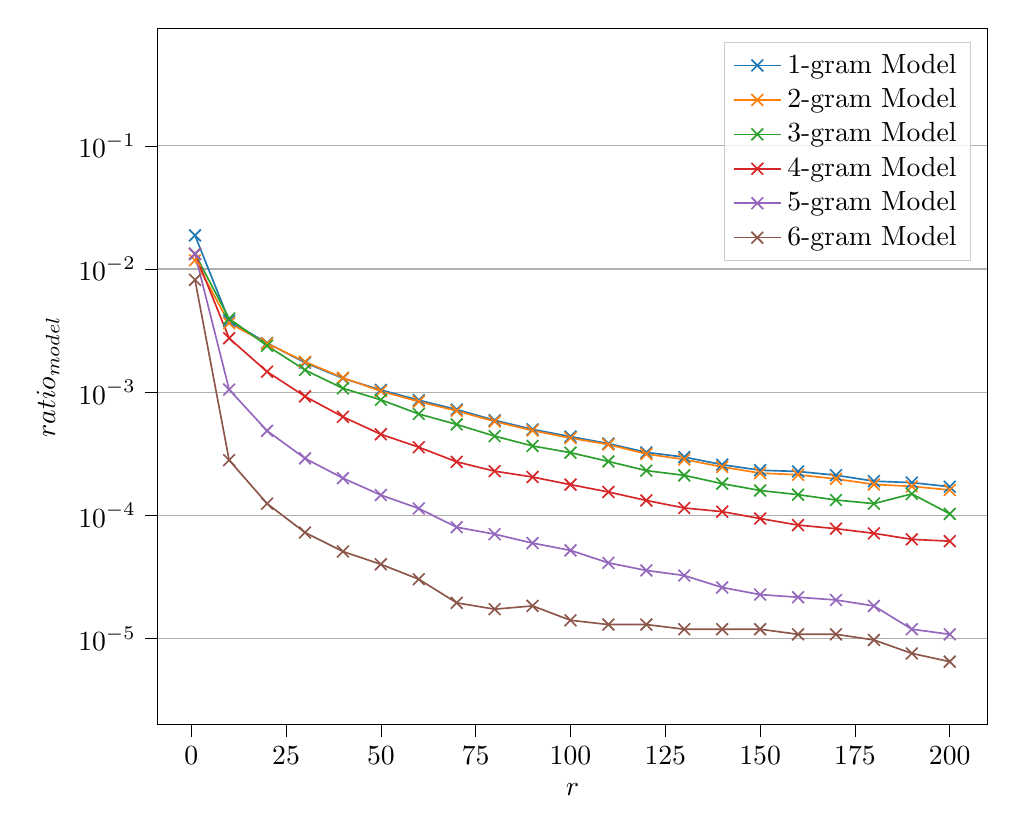
\begin{tikzpicture}

\definecolor{color0}{rgb}{0.12156862745098,0.466666666666667,0.705882352941177}
\definecolor{color1}{rgb}{1,0.498039215686275,0.0549019607843137}
\definecolor{color2}{rgb}{0.172549019607843,0.627450980392157,0.172549019607843}
\definecolor{color3}{rgb}{0.83921568627451,0.152941176470588,0.156862745098039}
\definecolor{color4}{rgb}{0.580392156862745,0.403921568627451,0.741176470588235}
\definecolor{color5}{rgb}{0.549019607843137,0.337254901960784,0.294117647058824}

\begin{groupplot}[group style={group size=2 by 1}]
%   \nextgroupplot[
%   height=.55\linewidth,
%   width=.5\linewidth,
%   legend cell align={left},
%   legend style={fill opacity=0.8, draw opacity=1, text opacity=1, draw=white!80!black},
%   log basis y={10},
%   tick align=outside,
%   tick pos=left,
%   title={Pruning ratios on 4-grams},
%   x grid style={white!69.0196078431373!black},
%   xlabel={\(\displaystyle r\)},
%   xmin=-8.95, xmax=209.95,
%   xtick style={color=black},
%   xtick={-25,0,25,50,75,100,125,150,175,200,225},
%   xticklabels={\(\displaystyle -25\),\(\displaystyle 0\),\(\displaystyle 25\),\(\displaystyle 50\),\(\displaystyle 75\),\(\displaystyle 100\),\(\displaystyle 125\),\(\displaystyle 150\),\(\displaystyle 175\),\(\displaystyle 200\),\(\displaystyle 225\)},
%   y grid style={white!69.0196078431373!black},
%       ylabel={\(\displaystyle ratio_{model}\)},
%   ymajorgrids,
%   ymin=2e-06, ymax=0.9,
%   yminorgrids,
%   ymode=log,
%   ytick style={color=black},
%   ytick={1e-07,1e-06,1e-05,0.0001,0.001,0.01,0.1,1,10},
%   yticklabels={\(\displaystyle 10^{-7}\),\(\displaystyle 10^{-6}\),\(\displaystyle 10^{-5}\),\(\displaystyle 10^{-4}\),\(\displaystyle 10^{-3}\),\(\displaystyle 10^{-2}\),\(\displaystyle 10^{-1}\),\(\displaystyle 10^{0}\),\(\displaystyle 10^{1}\)}
%   ]
%   \addplot [semithick, color0, mark=x, mark size=3, mark options={solid}]
%   table {%
%   1 0.0501147799247661
%   % 2 0.0370240812783332
%   % 3 0.0294929749541845
%   % 4 0.0210873549175321
%   % 5 0.0149734752274701
%   % 6 0.0153554319519017
%   % 7 0.0149734752274701
%   % 8 0.0149734752274701
%   % 9 0.0136835675015272
%   10 0.0102253801884062
%   20 0.00614860302864673
%   30 0.00433655917435616
%   40 0.00343503842073112
%   50 0.00279587178085716
%   60 0.00224672861138797
%   70 0.00183133459794871
%   80 0.00156512233546602
%   90 0.00137735909719316
%   100 0.00120502845384685
%   110 0.0010764234961258
%   120 0.000950390637559084
%   130 0.000853936919268272
%   140 0.000769057647172278
%   150 0.000691894672539606
%   160 0.000630164292833468
%   170 0.000583866508053865
%   180 0.000532424524965491
%   190 0.000498987235957982
%   200 0.00047455229399096
%   };
%   \addlegendentry{1-gram Model}
%   \addplot [semithick, color1, mark=x, mark size=3, mark options={solid}]
%   table {%
%   1 0.0526078367707091
%   % 2 0.038981849366847
%   % 3 0.0260238389716871
%   % 4 0.0260238389716871
%   % 5 0.0163078097541993
%   % 6 0.0158604262659962
%   % 7 0.0158604262659962
%   % 8 0.0158604262659962
%   % 9 0.0130645892870863
%   10 0.0108289111355113
%   20 0.00716433225845625
%   30 0.00448250990811905
%   40 0.00371167187581334
%   50 0.00281938347828892
%   60 0.00230507836027138
%   70 0.00175731242734667
%   80 0.00159620480001588
%   90 0.00136693625342976
%   100 0.00122317867827304
%   110 0.000943099264605674
%   120 0.000957970737897718
%   130 0.000861306161499265
%   140 0.000748530822367699
%   150 0.000698959244727404
%   160 0.000610969694415986
%   170 0.000583705326713924
%   180 0.000541569485719706
%   190 0.000506869381371455
%   200 0.00046969069814129
%   };
%   \addlegendentry{2-gram Model}
%   \addplot [semithick, color2, mark=x, mark size=3, mark options={solid}]
%   table {%
%   1 0.05397568317927
%   % 2 0.0400514844323416
%   % 3 0.0267995617440884
%   % 4 0.0213777404291079
%   % 5 0.017096235466817
%   % 6 0.014226297482156
%   % 7 0.0121988320267209
%   % 8 0.0107128040932252
%   % 9 0.0094448403876225
%   10 0.00839813209373574
%   20 0.00413790169026373
%   30 0.00260506972736652
%   40 0.00184237679371124
%   50 0.00137327277175592
%   60 0.00109032113946539
%   70 0.000858428448340054
%   80 0.00070844280866722
%   90 0.000589305279281804
%   100 0.000509525683711098
%   110 0.000455275558723156
%   120 0.000408471529321663
%   130 0.000366986139624936
%   140 0.000329755661691911
%   150 0.000296780095522808
%   160 0.000272314352881109
%   170 0.000243593698475708
%   180 0.000220191683774962
%   190 0.000196789669074215
%   200 0.000180833749960141
%   };
%   \addlegendentry{3-gram Model}

\nextgroupplot[
width=\linewidth,
height=.86\linewidth,
legend cell align={left},
legend style={fill opacity=0.8, draw opacity=1, text opacity=1, draw=white!80!black},
log basis y={10},
tick align=outside,
tick pos=left,
%title={Pruning ratios on 7-grams},
x grid style={white!69.0196078431373!black},
xlabel={\(\displaystyle r\)},
xmin=-8.95, xmax=209.95,
xtick style={color=black},
xtick={-25,0,25,50,75,100,125,150,175,200,225},
xticklabels={\(\displaystyle -25\),\(\displaystyle 0\),\(\displaystyle 25\),\(\displaystyle 50\),\(\displaystyle 75\),\(\displaystyle 100\),\(\displaystyle 125\),\(\displaystyle 150\),\(\displaystyle 175\),\(\displaystyle 200\),\(\displaystyle 225\)},
y grid style={white!69.0196078431373!black},
ylabel={\(\displaystyle ratio_{model}\)},
ymajorgrids,
ymin=2e-06, ymax=0.9,
yminorgrids,
ymode=log,
ytick style={color=black},
ytick={1e-07,1e-06,1e-05,0.0001,0.001,0.01,0.1,1,10},
yticklabels={\(\displaystyle 10^{-7}\),\(\displaystyle 10^{-6}\),\(\displaystyle 10^{-5}\),\(\displaystyle 10^{-4}\),\(\displaystyle 10^{-3}\),\(\displaystyle 10^{-2}\),\(\displaystyle 10^{-1}\),\(\displaystyle 10^{0}\),\(\displaystyle 10^{1}\)}
]
\addplot [semithick, color0, mark=x, mark size=3, mark options={solid}]
table {%
1 0.0187555820184578
% 2 0.0083015949601859
% 3 0.0083015949601859
% 4 0.00600548192709238
% 5 0.00500114634555304
% 6 0.00490019949834553
% 7 0.00490019949834553
% 8 0.00458196028511493
% 9 0.00400023269103766
10 0.00379491706959856
20 0.00250827250858043
30 0.00174004989169596
40 0.00129691034209001
50 0.00104368774231522
60 0.000862325610044068
70 0.000723737565572646
80 0.000591993375149258
90 0.000499601345501755
100 0.000436295695558031
110 0.000383255826686191
120 0.00032508306727852
130 0.000297707651086609
140 0.000258355490310835
150 0.000232691037630905
160 0.000227558147094964
170 0.000212159475487028
180 0.00018991694983117
190 0.000184784059295118
200 0.000171096351199163
};
\addlegendentry{1-gram Model}
\addplot [semithick, color1, mark=x, mark size=3, mark options={solid}]
table {%
1 0.0117808735000346
% 2 0.00865904661981776
% 3 0.00865904661981776
% 4 0.00716893750070402
% 5 0.00556457595453075
% 6 0.00501906084504955
% 7 0.00467147599653062
% 8 0.00435285655205486
% 9 0.00405676575516833
10 0.00363998577476821
20 0.00249102474771934
30 0.0017684988357517
40 0.00131148912751378
50 0.0010202258979678
60 0.00083999671725421
70 0.000706434020832591
80 0.000579308080864926
90 0.000489193490508244
100 0.000424825925967598
110 0.000376550252562224
120 0.000315401066248722
130 0.000284826473091915
140 0.000247815123481154
150 0.00022045890855138
160 0.000214022152097315
170 0.000197930260962154
180 0.000178619991600071
190 0.000172183235146006
200 0.000160918911351393
};
\addlegendentry{2-gram Model}
\addplot [semithick, color2, mark=x, mark size=3, mark options={solid}]
table {%
1 0.0132758052057387
% 2 0.00971410965205388
% 3 0.00965444067384724
% 4 0.00675669811402635
% 5 0.00599402008349315
% 6 0.00536152891450192
% 7 0.00493842161449065
% 8 0.00454677613935206
% 9 0.00420178095626589
10 0.0039598503719005
20 0.00238458934724306
30 0.00151559204645069
40 0.00107512649823382
50 0.000867912410279503
60 0.000666122774889533
70 0.000547869708989013
80 0.000440465548216862
90 0.000366692993343132
100 0.000323297372829101
110 0.000274477299750941
120 0.000231081679236911
130 0.000211553650005691
140 0.000181176715645881
150 0.000159478905388921
160 0.000147545109747571
170 0.000133441533080481
180 0.000124762408977741
190 0.0001497148907732
200 0.00010306459872067
};
\addlegendentry{3-gram Model}
\addplot [semithick, color3, mark=x, mark size=3, mark options={solid}]
table {%
1 0.0132758052057387
% 2 0.00971410965205388
% 3 0.00693028059608225
% 4 0.00553728117758356
% 5 0.00493408205243928
% 6 0.00422564854754859
% 7 0.00371032555394513
% 8 0.00341306555342435
% 9 0.00289448788828228
10 0.00274477299750908
20 0.00146785686388529
30 0.000925411607460624
40 0.000631406278478353
50 0.000455654015396711
60 0.000358013869240281
70 0.000272307518725201
80 0.000228911898211281
90 0.000205044306928581
100 0.00017792204410727
110 0.00015513934333744
120 0.00013235664256761
130 0.00011499839436202
140 0.00010740416077204
150 9.43854746179307e-05
160 8.35365694894508e-05
170 7.81121169252108e-05
180 7.16027738481007e-05
190 6.40085402581203e-05
200 6.18387592323799e-05
};
\addlegendentry{4-gram Model}
\addplot [semithick, color4, mark=x, mark size=3, mark options={solid}]
table {%
1 0.0132758052057387
% 2 0.00616109322247194
% 3 0.00373310825471496
% 4 0.00264604796083978
% 5 0.00223161978493136
% 6 0.00178030533158591
% 7 0.00155681788593898
% 8 0.00132356642567633
% 9 0.00125847299490534
10 0.00105125890695112
20 0.000486030949756522
30 0.000290750657443661
40 0.0002007047448771
50 0.000146460219234701
60 0.00011391350384915
70 8.02818979508402e-05
80 7.05178833352305e-05
90 5.96689782067505e-05
100 5.20747446167702e-05
110 4.12258394882903e-05
120 3.58013869240503e-05
130 3.25467153854397e-05
140 2.60373723084406e-05
150 2.278270076983e-05
160 2.16978102569598e-05
170 2.06129197440896e-05
180 1.84431387184603e-05
190 1.19337956413501e-05
200 1.08489051284799e-05
};
\addlegendentry{5-gram Model}
\addplot [semithick, color5, mark=x, mark size=3, mark options={solid}]
table {%
1 0.00817248023329487
% 2 0.00253864380006774
% 3 0.00133441533080481
% 4 0.000875506643869484
% 5 0.000642255183606832
% 6 0.000534851022834792
% 7 0.000426361971549882
% 8 0.000378626788984482
% 9 0.000325467153854841
10 0.000280986642828052
20 0.000124762408977741
30 7.26876643608598e-05
40 5.09898541039e-05
50 4.01409489754201e-05
60 3.03769343598104e-05
70 1.95280292313305e-05
80 1.73582482055901e-05
90 1.84431387184603e-05
100 1.41035766670905e-05
110 1.30186861542203e-05
120 1.30186861542203e-05
130 1.19337956413501e-05
140 1.19337956413501e-05
150 1.19337956413501e-05
160 1.08489051284799e-05
170 1.08489051284799e-05
180 9.76401461560972e-06
190 7.59423358998035e-06
200 6.50934307711015e-06
};
\addlegendentry{6-gram Model}
\end{groupplot}

\end{tikzpicture}

    %\caption{Pruning ratios on 7-grams}
    \end{figure}
\end{columns}
\end{frame}

\begin{frame}[fragile]{Comparison and Combination with Frequency Pruning}
\vspace{1cm}
    \begin{center}
    Pruning ratios on 5-grams
    \end{center}
%\begin{figure}[H]
\centering% \includegraphics[width=\textwidth/2]{plots/ex2.png}
% This file was created by tikzplotlib v0.9.3.
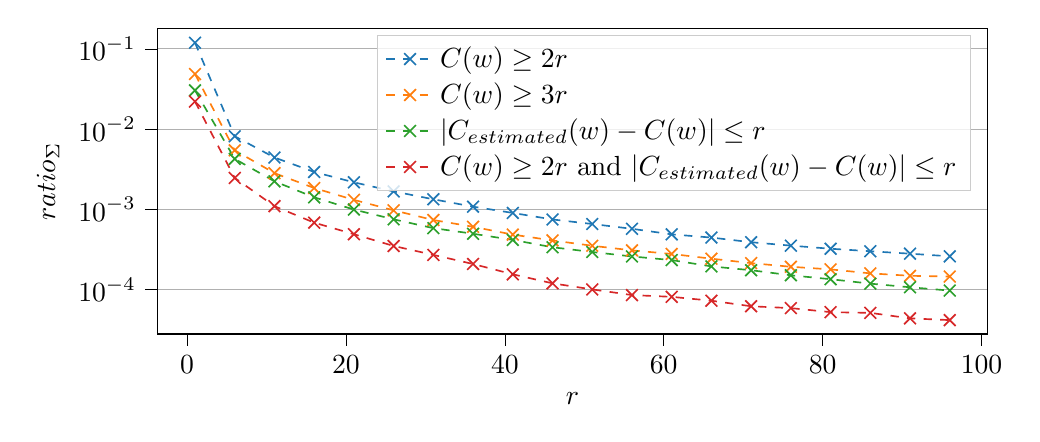
\begin{tikzpicture}

\definecolor{color0}{rgb}{0.12156862745098,0.466666666666667,0.705882352941177}
\definecolor{color1}{rgb}{1,0.498039215686275,0.0549019607843137}
\definecolor{color2}{rgb}{0.172549019607843,0.627450980392157,0.172549019607843}
\definecolor{color3}{rgb}{0.83921568627451,0.152941176470588,0.156862745098039}

\begin{axis}[
width=\textwidth,
height=.45\textwidth,
legend cell align={left},
legend style={fill opacity=0.8, draw opacity=1, text opacity=1, draw=white!80!black},
log basis y={10},
tick align=outside,
tick pos=left,
x grid style={white!69.0196078431373!black},
xlabel={\(\displaystyle r\)},
xmin=-3.75, xmax=100.75,
xtick style={color=black},
xtick={-20,0,20,40,60,80,100,120},
xticklabels={\(\displaystyle -20\),\(\displaystyle 0\),\(\displaystyle 20\),\(\displaystyle 40\),\(\displaystyle 60\),\(\displaystyle 80\),\(\displaystyle 100\),\(\displaystyle 120\)},
y grid style={white!69.0196078431373!black},
ylabel={\(\displaystyle ratio_\Sigma\)},
ymajorgrids,
ymin=2.81102688510379e-05, ymax=0.177368374755121,
ymode=log,
ytick style={color=black},
ytick={1e-06,1e-05,0.0001,0.001,0.01,0.1,1,10},
yticklabels={\(\displaystyle 10^{-6}\),\(\displaystyle 10^{-5}\),\(\displaystyle 10^{-4}\),\(\displaystyle 10^{-3}\),\(\displaystyle 10^{-2}\),\(\displaystyle 10^{-1}\),\(\displaystyle 10^{0}\),\(\displaystyle 10^{1}\)}
]
\addplot [semithick, color0, dashed, mark=x, mark size=3, mark options={solid}]
table {%
1 0.119164914388705
6 0.008149165343518
11 0.00443183281122602
16 0.00292880744968459
21 0.00217568553405141
26 0.00167789554992919
31 0.00133781058232846
36 0.00108247865081749
41 0.000904389992704802
46 0.000749903445908252
51 0.000658713470368622
56 0.000573960434278848
61 0.000489207398189074
66 0.000446294468523366
71 0.000390507659957945
76 0.000354031669742093
81 0.000323992618976097
86 0.000301463330901601
91 0.000281079689310389
96 0.000260696047719178
};
\addlegendentry{$C(w) \geq 2r$}
\addplot [semithick, color1, dashed, mark=x, mark size=3, mark options={solid}]
table {%
1 0.0485967471999313
6 0.00544672359782002
11 0.0028311805346951
16 0.00184847444535038
21 0.00131528129425396
26 0.000975196326653221
31 0.000738102390250182
36 0.000608290778011415
41 0.000485988928464146
46 0.000410891301549157
51 0.000352958846500451
56 0.0003089730935931
61 0.000278934042827104
66 0.000243530875852894
71 0.000214564648328541
76 0.000193108183495687
81 0.000179161481354332
86 0.000159850663004763
91 0.000149122430588336
96 0.000145903960863408
};
\addlegendentry{$C(w) \geq 3r$}
\addplot [semithick, color2, dashed, mark=x, mark size=3, mark options={solid}]
table {%
1 0.0304005921984294
6 0.00426232673904647
11 0.00223898210530837
16 0.00141505385572671
21 0.000996652791486086
26 0.000753121915633148
31 0.000584688666695254
36 0.000497789984122199
41 0.000417328240999049
46 0.000337939321117475
51 0.000295026391451736
56 0.00025962322447759
61 0.00023387546667808
66 0.000195253829978981
71 0.000174870188387799
76 0.000151268077071665
81 0.000135175728447012
86 0.00011908337982236
91 0.000107282324164237
96 9.76269149894904e-05
};
\addlegendentry{$|C_{estimated}(w)-C(w)| \leq r$}
\addplot [semithick, color3, dashed, mark=x, mark size=3, mark options={solid}]
table {%
1 0.0220615371411406
6 0.00246749345577823
11 0.00109749817620049
16 0.000684461228168047
21 0.00049135304467236
26 0.000350813200017165
31 0.000271424280135605
36 0.000209200532120328
41 0.000155559370038193
46 0.000120156203063983
51 0.000100845384714414
56 8.58258593314166e-05
61 8.15345663648457e-05
66 7.29519804317041e-05
71 6.2223748015277e-05
76 5.90052782903489e-05
81 5.25683388404927e-05
86 5.14955155988499e-05
91 4.3985752907351e-05
96 4.18401064240656e-05
};
\addlegendentry{$C(w) \geq 2r$ and $|C_{estimated}(w)-C(w)| \leq r$ }
\end{axis}

\end{tikzpicture}

%\end{figure}
\end{frame}

\begin{frame}[fragile]{Comparison and Combination with Frequency Pruning}
\vspace{1cm}
\begin{columns}
    \column{.4\linewidth}
    \begin{itemize}
        \item The table shows which ratio of the N-grams \emph{after} frequency pruning
            remain after model pruning with tolerance $r$
        \begin{itemize}
            \item Our approach shows great potential over a wide range of
                $(r,threshold)$-combinations.
            \item Even at a high threshold of $100$ combined with smaller values for $r$, we
                can prune about half of all remaining N-grams
        \end{itemize}
    \end{itemize}
    \column{.6\linewidth}
       \begin{figure}[H]
       \centering% \includegraphics[width=\textwidth/2]{plots/ex2.png}
       \input{../thesis/table_improvement_ratios_5_triangle.tex}
       \caption*{Ratio of combined approach compared to frequency pruning on a 5-gram corpus.} 
       \end{figure}
\end{columns}
\end{frame}

\begin{frame}{End-to-End Evaluation}
    \begin{columns}
    \column{.5\linewidth}
    \begin{itemize}
        \item Previous Experiments:
            \begin{itemize}
                \item Work on precomputed values of $P_{N-gram}(w)$
                \item But pruning introduces noise into $P_{N-gram}(w)$
            \end{itemize}
        \item This Experiment:
            \begin{itemize}
                \item Build a sample corpus from 7-grams and their sub-N-grams 
                    ($\approx 1.8$M N-grams)
                \item Extend our model into a working system, and prune said corpus
            \end{itemize}
        \item Results
                \begin{itemize}
                    \item Pruning ratio worsens from $\approx .2-.3$ to $\approx .3-.4$
                    \item Still a significant improvement!
                \end{itemize}
    \end{itemize}
    \column{.5\linewidth}
        \begin{figure}
        \begin{tabular}[]{cccc}
\toprule
threshold & r & $ratio_{actual}$ & $ratio_{predicted}$ \\
\midrule
\phantom{0}2  & 1  & 0.40 & 0.19 \\
\phantom{0}4  & 2  & 0.30 & 0.33 \\
           10 & 5  & 0.31 & 0.33 \\
           20 & 10 & 0.33 & 0.29 \\
           40 & 20 & 0.34 & 0.26 \\
           80 & 40 & 0.34 & 0.21 \\
\bottomrule
\end{tabular}

            \caption*{Improvement over thresholding in end-to-end pruning on a 5-gram corpus.}
        \end{figure}
    \end{columns}
\end{frame}

\section{Conclusion}
\subsection{Conclusion}

\begin{frame}{Conclusion}
\begin{itemize}
    \item We developed a pruning algorithm that reduced frequency pruned corpora to $\approx 30-40\%$ of their size.
    \item Further Work 
    \begin{itemize}
        \item Combination with Compression
        \item Representation of Time
    \end{itemize}
    \item Lessons Learned
    \begin{itemize}
        \item N-gram NLP is a facinatingly well-studied subject
        \begin{itemize}
            \item Culturomics is mostly unstudied on a technical level
        \item NLP methods can be useful for other N-gram applications
        \end{itemize}
%       \item Taco Bell Programming is great for Big Data
%       \item Python + PyPy/Numba can get you very far
%       \item Jupyter Notebooks are easy to get wrong
    \end{itemize}
\end{itemize}
\end{frame}
\appendix
\beginbackup{}

\begin{frame}[allowframebreaks]{References}
\printbibliography{}
\end{frame}

\begin{frame}{Example: Calculating $P_{N-gram}(w)$}
\begin{itemize}
    \item Example: Estimating $P(I\ am\ Brian)$ using a 2-gram corpus
\begin{equation*}
\begin{aligned}
P(I\ am\ Brian) &=       P(I)                                        \cdot P(am|I)                        \cdot P(Brian|I\ am)             \qquad &&  \text{Chain Rule} \\
                &\approx P(I)                                        \cdot P(am|I)                        \cdot P(Brian| am)                      &&  \text{Markov Assumption} \\
%                &=       P(I)                                        \cdot \frac {Count(I\ am)} {Count(I)}        \cdot \frac {Count(am\ Brian)}{Count(am)}       &&  \text{MLE} \\
                &= \frac {Count(I)} {\sum_{w \in corpus, |w| = 1} Count(w) } \cdot \frac {Count(I\ am)} {Count(I)}        \cdot \frac {Count(am\ Brian)}{Count(am)}       &&  \text{MLE} 
\end{aligned}
\end{equation*}
\end{itemize}


\end{frame}
\begin{frame}{Pruning}
\vspace{.9cm}
    \begin{itemize}
        \item We prune N-grams by ascending length (1-grams first, then 2-grams, \ldots)
        \item For each length, we take a sample of N-grams and build our linear models
            $C_{estimated}(w) = slope \cdot P_{N-gram}(w) + intercept$ using RANSAC
        \item We then divide N-grams in three mutually exclusive cases:
\begin{enumerate}
\def\labelenumi{\arabic{enumi}.}
% \item The N-gram is unknown (i.e.~has \(C(w) = 0\)).
\item $Count(w) < threshold$
    \begin{itemize}
            \item Add to $Bloom\_Filter_{threshold}$ and remove from corpus
    \end{itemize}
\item Our estimation error is $\leq r$, so we can estimate its count when it is queried.
    \begin{itemize}
            \item Add to $Bloom\_Filter_{model}$ and remove from corpus
    \end{itemize}
\item Otherwise
    \begin{itemize}
        \item Keep in Corpus
    \end{itemize}
\end{enumerate}
\end{itemize}
    %\vspace{1cm}
    \begin{block}{RANSAC}
    RANSAC is a probablistic algorithm for robust linear fits. It's commonly used in Computer Vision.
    \end{block}
    \begin{block}{Bloom Filters}
    A Bloom filter is a space efficent set data structure, that allows membership queries.
    They have a user-chosen chance $\epsilon$ of falsely returning $\in$. This is called a \emph{collision}.
    \end{block}

\end{frame}

\begin{frame}[fragile]{Pruning}
\vspace{1cm}
\def\set#1#2{\left\{#1 \ \mid{} \ #2 \right\} }
\begin{algorithm}[H]
\begin{algorithmic}[1]
\Procedure{pruning}{$corpus, r, threshold$}
\For{$n \gets 1,\ldots \max_w |w|$}
    \State{$model\_pruned, thresh\_pruned \gets \emptyset$}
    \State{$ngrams \gets \left\{w \in corpus \ \mid \  |w| = n  \right\} $}
    \State{$thresh\_pruned \gets \left\{w \in ngrams \ \mid \ C(w) < threshold \right\} $}
    \State{$estimates \gets \left\{(P_{N-gram}(w), C(w))  \ \mid \  w \in ngrams \setminus thresh\_pruned  \right\} $ }
    \State{$model \gets fit\_linear\_model(estimates, r)$}
    \State{$model\_pruned \gets \left\{w \in ngrams \setminus thresh\_pruned  \ \mid \  r \leq |C(w) - model.estimateCount(w)| \right\} $}
    \State{$unpruned \gets ngrams \setminus (thresh\_pruned \cup model\_pruned)$}
    \State{$result[n] \gets (bloom\_filter(thresh\_pruned), model, bloom\_filter(model\_pruned), unpruned)$}
\EndFor{}
\State{\textbf{return} $result$}
\EndProcedure{}
\end{algorithmic}
\end{algorithm}
\end{frame}

\subsection{A model-based Pruning Approach}
\begin{frame}{Querying}
    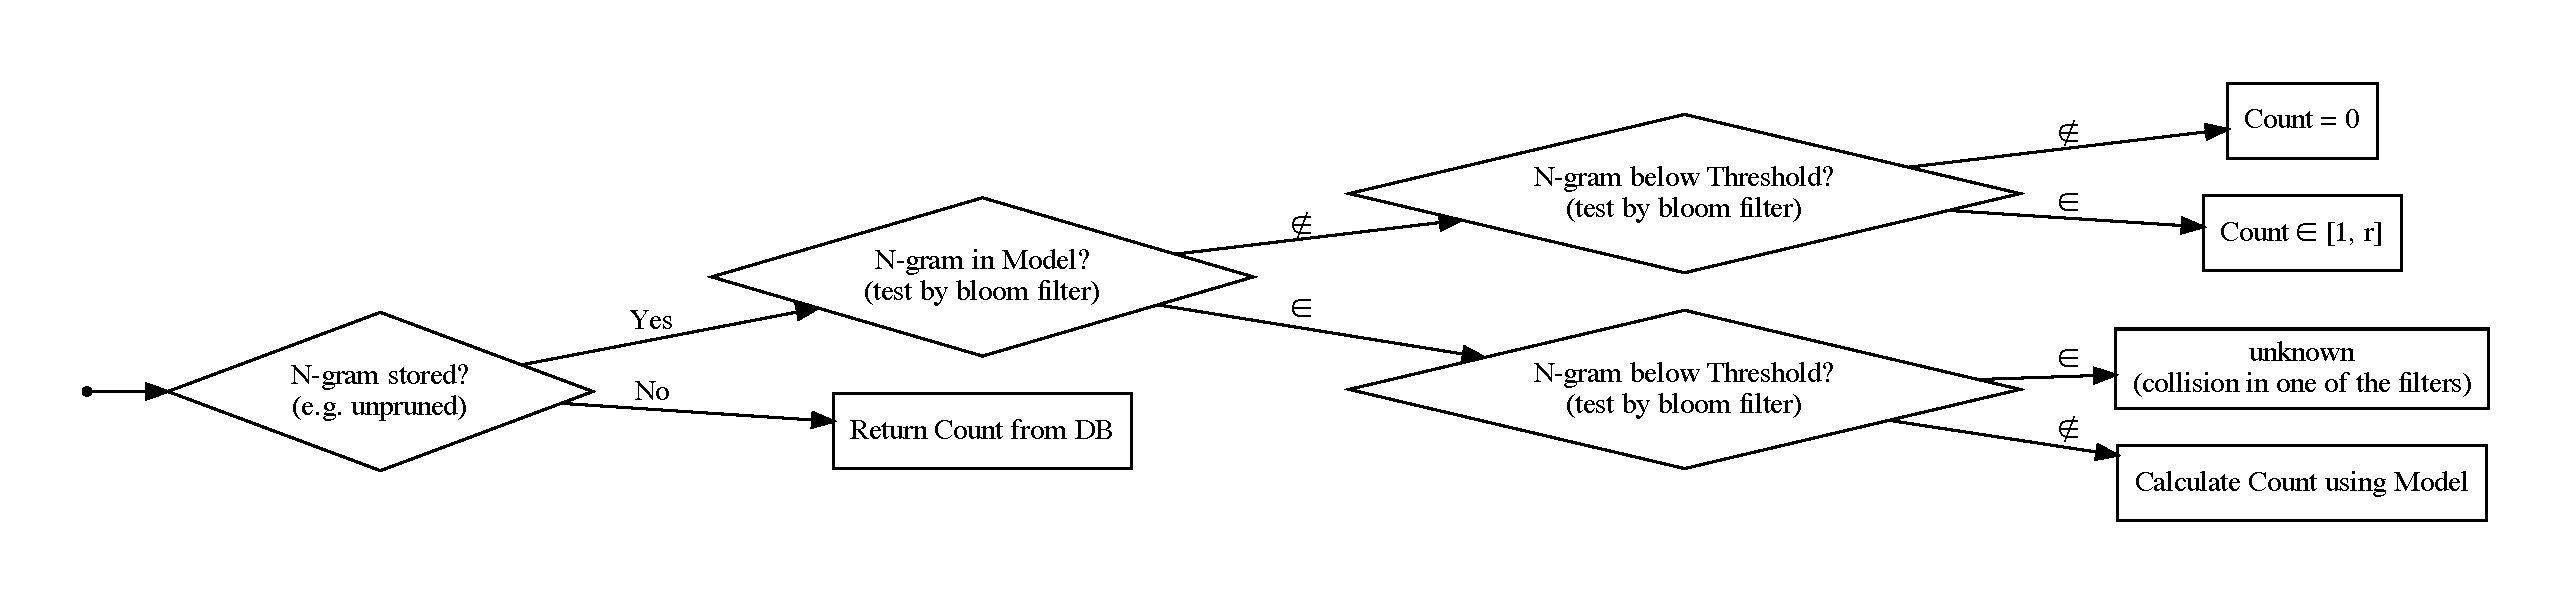
\includegraphics[width=\textwidth]{Interpretation.pdf}
\end{frame}
\begin{frame}[fragile]{N-gram Models: Problems}
\vspace{1cm}
\begin{itemize}

\item Problems:
\begin{itemize}
\item small N $\rightarrow$ little context
\item high N $\rightarrow$ little generality, very high storage requirements
\end{itemize}
\end{itemize}

\lstset{
frame = single,  
framexleftmargin=1pt}
\begin{columns}

\column{0.2\textwidth}
\begin{lstlisting}[title={2-grams.txt}]
and if        5 
and in        7 
and wondering 2
and butter    6
and knocked   1
\end{lstlisting}

\column{0.34\textwidth}
\begin{lstlisting}[title={5-grams.txt}]
to the door and knocked 1
to the door and tried   1
the door and tried to   1
and tried to open it    1
tried to open it but    1
\end{lstlisting}
\column{0.45\textwidth}
    \begin{figure}[H]
    % This file was created by tikzplotlib v0.9.3.
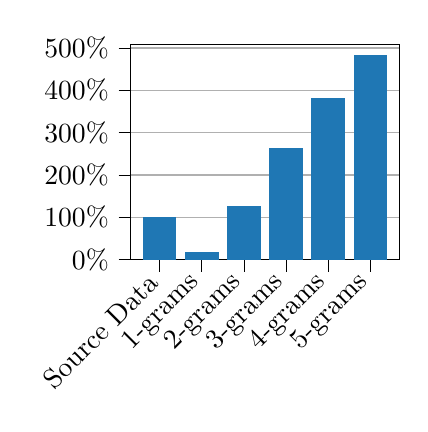
\begin{tikzpicture}

\definecolor{color0}{rgb}{0.12156862745098,0.466666666666667,0.705882352941177}

\begin{axis}[
width=5cm,
tick align=outside,
tick pos=left,
title={},
x grid style={white!69.0196078431373!black},
xmin=-0.69, xmax=5.69,
xtick style={color=black},
xtick={0,1,2,3,4,5},
xticklabel style={
    rotate=45,
    anchor=east,
},
xticklabels={Source
 Data,1-grams,2-grams,3-grams,4-grams,5-grams},
y grid style={white!69.0196078431373!black},
ymajorgrids,
ymin=0, ymax=5.07972972972973,
ytick style={color=black},
ytick={0,1,2,3,4,5,6},
yticklabels={0\%,100\%,200\%,300\%,400\%,500\%,600\%}
]
\draw[draw=none,fill=color0] (axis cs:-0.4,0) rectangle (axis cs:0.4,1);
\draw[draw=none,fill=color0] (axis cs:0.6,0) rectangle (axis cs:1.4,0.189189189189189);
\draw[draw=none,fill=color0] (axis cs:1.6,0) rectangle (axis cs:2.4,1.27027027027027);
\draw[draw=none,fill=color0] (axis cs:2.6,0) rectangle (axis cs:3.4,2.64864864864865);
\draw[draw=none,fill=color0] (axis cs:3.6,0) rectangle (axis cs:4.4,3.81081081081081);
\draw[draw=none,fill=color0] (axis cs:4.6,0) rectangle (axis cs:5.4,4.83783783783784);
\end{axis}

\end{tikzpicture}

        \caption*{Space needed for a text corpus and its N-grams}
    \end{figure}
\end{columns}

\end{frame}
\begin{frame}{N-gram Models in Practice}
\vspace{1cm}
\begin{itemize}
	\item N-gram creation
	\item pruning
	\begin{itemize}
		\item by frequency (e.g.\ remove all N-grams with $counts < 40$)
		\item by entropy (\cite{Stolcke98})
	\end{itemize}
\item compression
	\begin{itemize}
		\item using Bloom filters (\cite{Talbot07})
        \begin{itemize}
                \item
        \end{itemize}
		\item using Tries
		\item \dots
	\end{itemize}
	\item {interpretation}
	\begin{itemize}
		\item backoff (falling back to lower N-grams)
		\item interpolation (mixing the estimates of different N-Gram models)
		\item smoothing (accounting for unknown N-grams)
		\end{itemize}
	\item application
	
\end{itemize}
\end{frame}
\backupend{}

\end{document}
